
\section{The Narrator Agent}
\label{sec:narrator}

The Narrator serves as the sole truth-keeper in the game: it holds beliefs about the current state of the game, along with the complete \emph{log} (see Subsection \ref{subsec:logging}), which can be used as context by other agents when needed. It orchestrates all game interactions by simulating a \textbf{graph traversal} on its internal state machine.

\subsection{Setup and Settings Configuration}
\label{subsec:narrator-setup}

At the start of the MAS simulation, the Narrator is the only agent that "wakes up". Its first task is to define the simulation's settings, along with verifying everything is coherent such as "pinging" the \emph{Ollama bridge} (Section \ref{sec:llm}) to verify that it is correctly set up and available.

The code regarding this part is defined in the file \texttt{narrator/init\_narrator.asl}, where the baseline configuration is defined by a hard-coded schema containing default values and scope annotations (either \texttt{[local]} for Narrator-exclusive settings or \texttt{[share]} for settings that must be broadcast to all players, such as the inability to utilize the LLM if the ping fails). 

However, those parameters can be easily tinkered by the user, directly by editing the \texttt{werewolf.jcm} file without modifying the underlying agent's code (Listing \ref{lst:jcm_setup} propose a example of a custom configuration).

During the \texttt{setup} execution, the Narrator parses these overriding beliefs. Any setting provided in the \texttt{werewolf.jcm} file that does not exist in the predefined whitelist is immediately rejected and abolished to prevent logical errors; the accepted settings are then updated. 

\vspace{1em}
\begin{lstlisting}[frame=single, language=Prolog, caption={Example configuration in the \texttt{werewolf.jcm} file overriding the default Narrator settings: is defined a  specific LLM model, the maximum number of rounds to hunt or speak is changed and all the \emph{artificial} delays are removed.}, label={lst:jcm_setup}]
agent narrator : narrator.asl {
    beliefs:  setting(llm_model("gemma4:31b")),
              setting(max_hunt_rounds(5)),
              setting(max_discussion_turns(10)),
              setting(disable_delay(true))
}
\end{lstlisting}

Once the Narrator's configuration is fully set up, it broadcasts the \texttt{[share]} settings to all active players and waits for them to acknowledge their configurations before officially starting the game.


\subsection{The Game Graph}
\label{subsec:game-graph}

The flow of a Werewolf game is inherently cyclical and phase-based (e.g., Night falls, Wolves hunt, Day breaks, Village discusses, Village votes). To formally define the execution of the state machine, the Narrator relies on a directed multi-edge graph engine defined within the \texttt{game\_graph.asl} file. 

\begin{figure}[H]
    \centering
    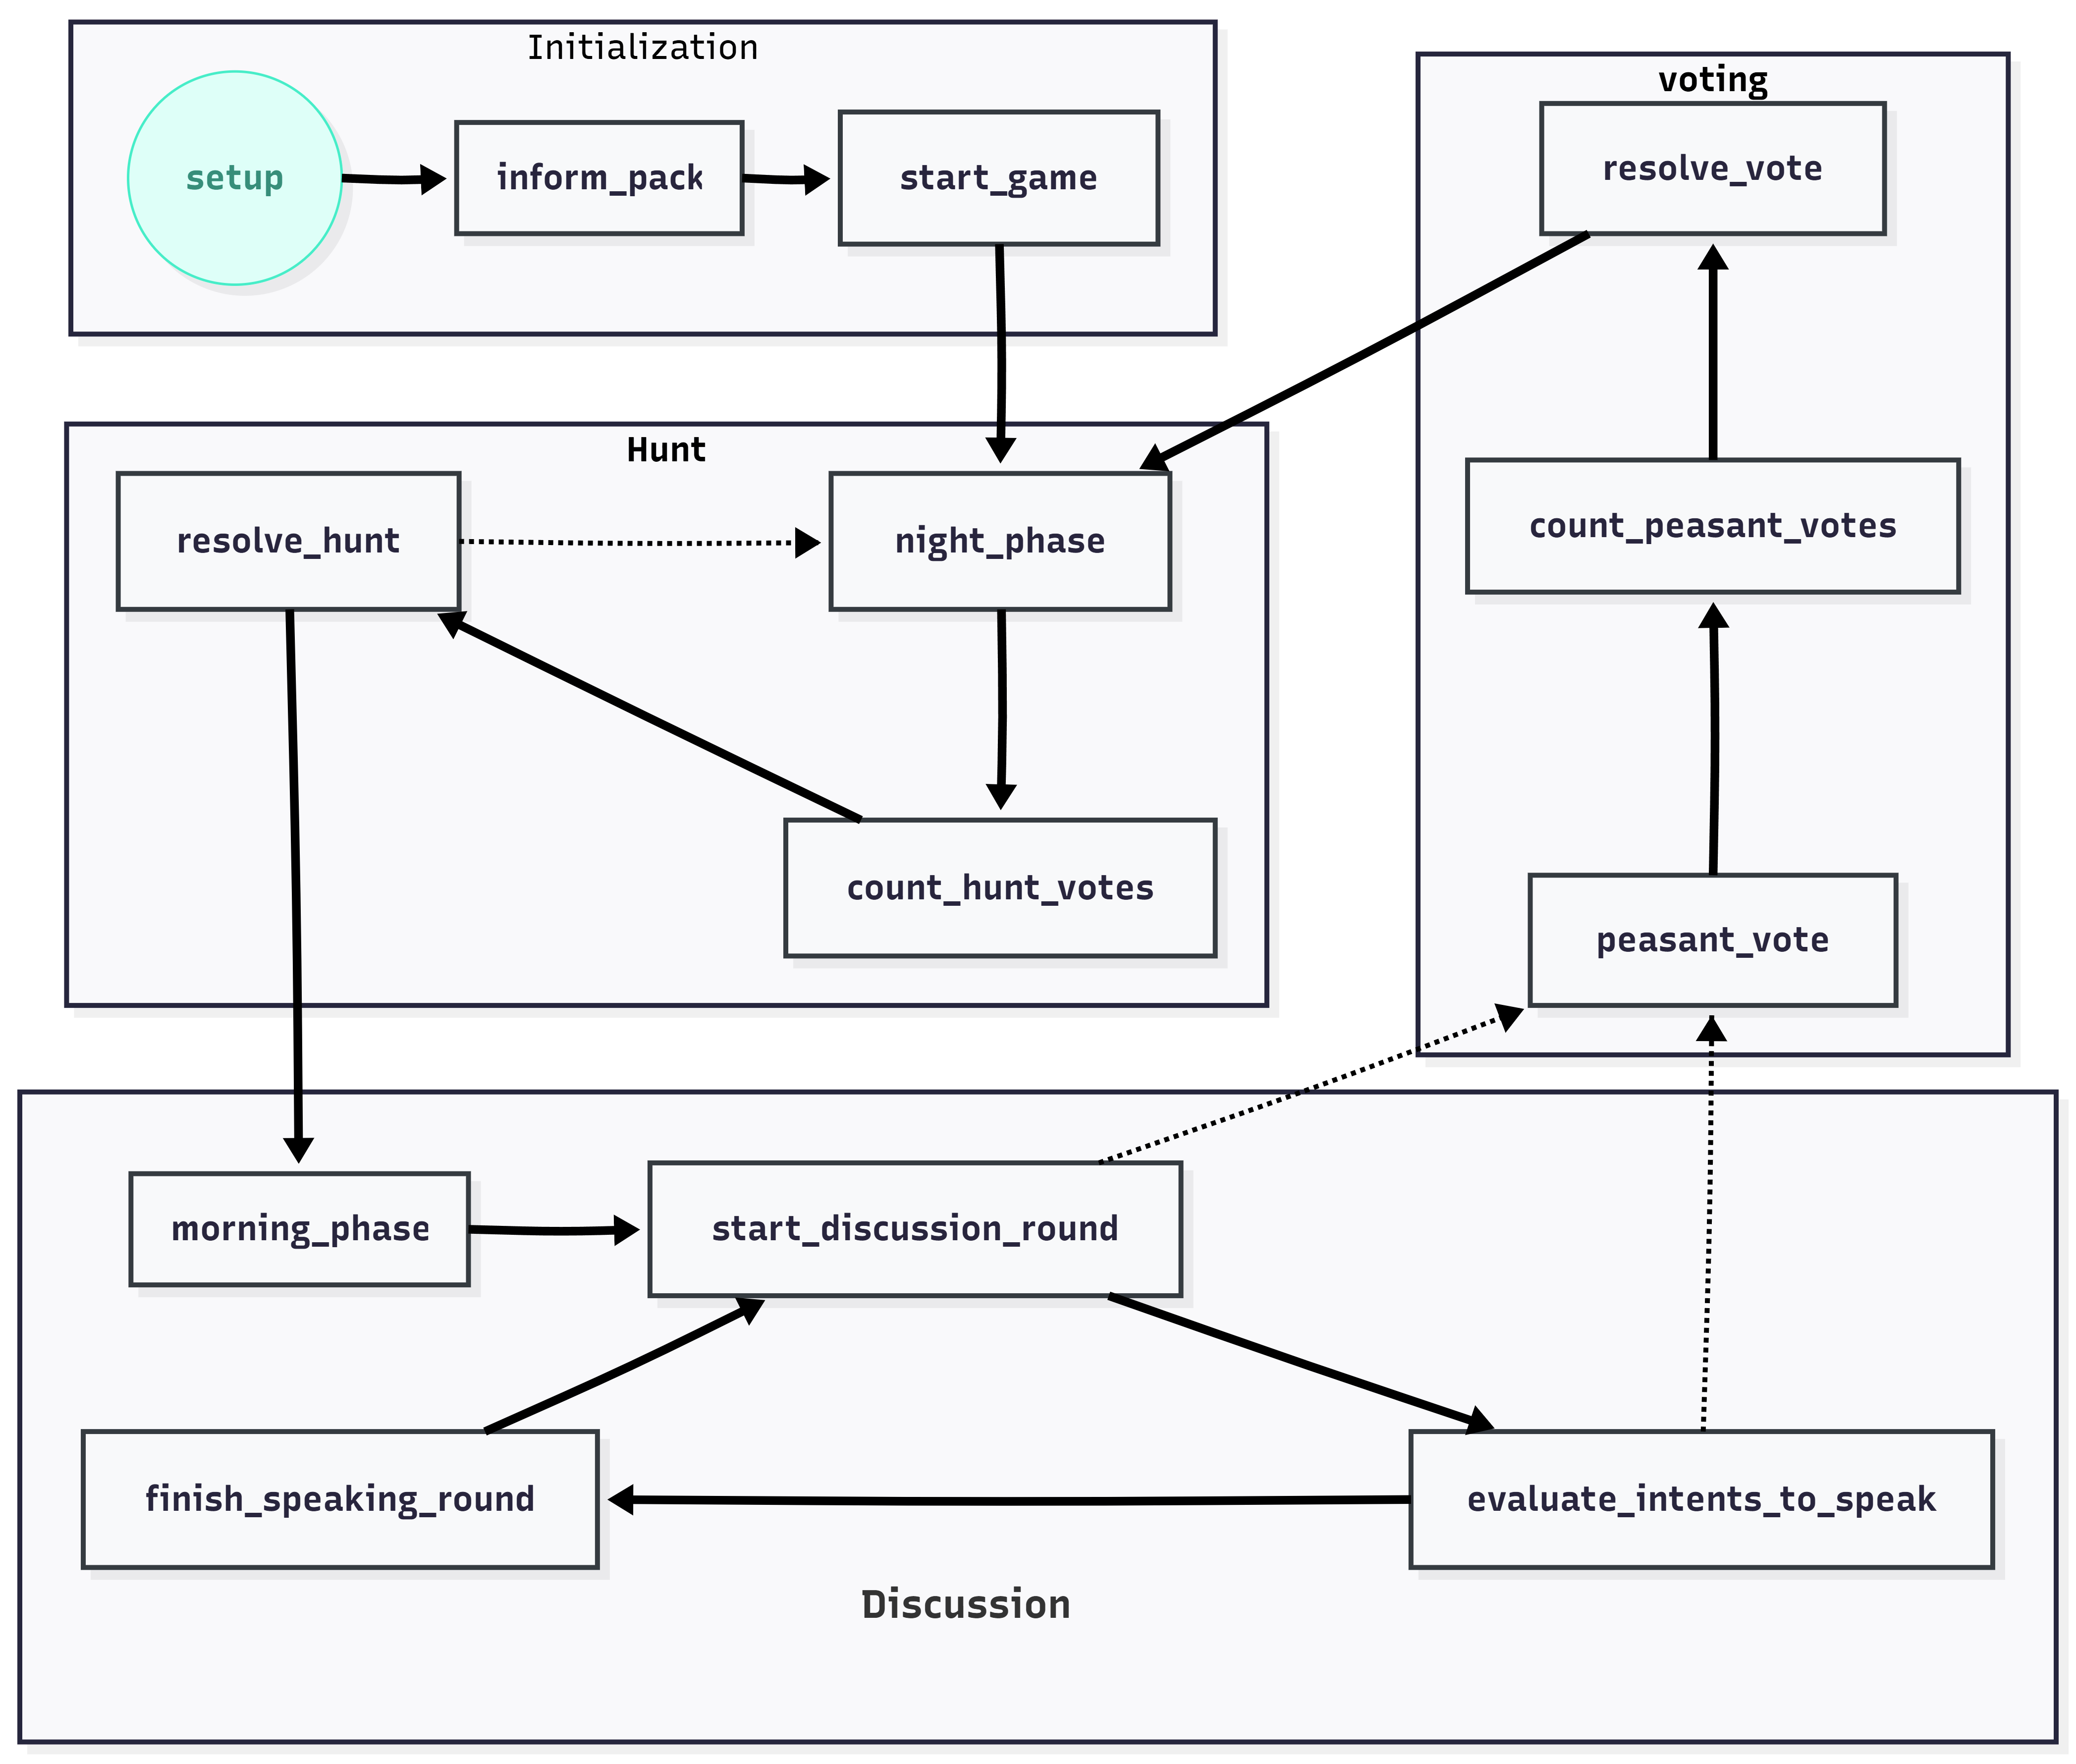
\includegraphics[width=\textwidth]{images/full_game_graph.png}
    \caption{Symplified visualization of the state machine representing the game phases and transitions.}
    \label{fig:master_graph}
\end{figure}

The graph is formalized using rule-based beliefs natively implemented in Jason, allowing the engine to represent complex game states and conditional branching within a  ``user-readable`` implementation. 

\subsubsection{Nodes}
Every state in the game is represented as a node structured as a triplet $$\texttt{node(EnterAction, NodeName, CleanUpList)}$$ 

The \texttt{EnterAction}, if defined, is an \texttt{action(Audience, ActionName)} that is broadcast to all players within the \texttt{Audience} (a subset of the alive players), who must then respond to, to release a \texttt{sync\_barrier} set up to synchronize them (see Subsection \ref{subsec:sync-barrier}).

On the other hand, \texttt{CleanUpList} is a list of beliefs that are abolished once the Narrator leaves the node (since they fulfill their purpose). This prevents the belief base from becoming cluttered and mitigates the risk of invalid states.

\vspace{1em}
\begin{lstlisting}[frame=single, language=Prolog, caption={Example of a node definition representing the Daytime Voting Phase: to every player is injected the goal \texttt{choose\_vote}, and from the narrator itself is abolishe the  belief about the last person who spoke.}, label={lst:peasant_vote_node}]
node(
    action(TargetList, choose_vote), 
    peasant_vote, 
    [last_speaker(_)]
) :- players(TargetList).
\end{lstlisting}

\subsubsection{Edges}

The transitions are modeled as a multi-edge graph, meaning multiple distinct paths can exist between the same two nodes depending on the game's context (e.g., a tied vote versus a decisive execution). An edge is defined as $$\texttt{edge(FromNode, Message, ToNode)}$$ 

Each \texttt{Message} is further defined as a complex structure \footnote{Each on of those ``structures`` are actually Jason's beliefs, each time verified on-the-fly to ensure a graph traversal coherent witht the current game's state.} defined as $$\texttt{msg(Players, PhaseMsg, PhaseTitle, Action)}$$ which describes exactly what is broadcast to all players (or a subset of them) during the transition:
\begin{itemize}
    \item \textbf{\texttt{Players}:} The target audience receiving the transition message.
    \item \textbf{\texttt{PhaseMsg} \& \texttt{PhaseTitle}:} Narrative text elements, mainly used to update the LLM context or the UI.
    \item \textbf{\texttt{Action}:} is the actual \emph{speech-act} of the message, i.e. the actual logic information that the players use to  update their belief base.
\end{itemize}

\begin{figure}[H]
    \centering
    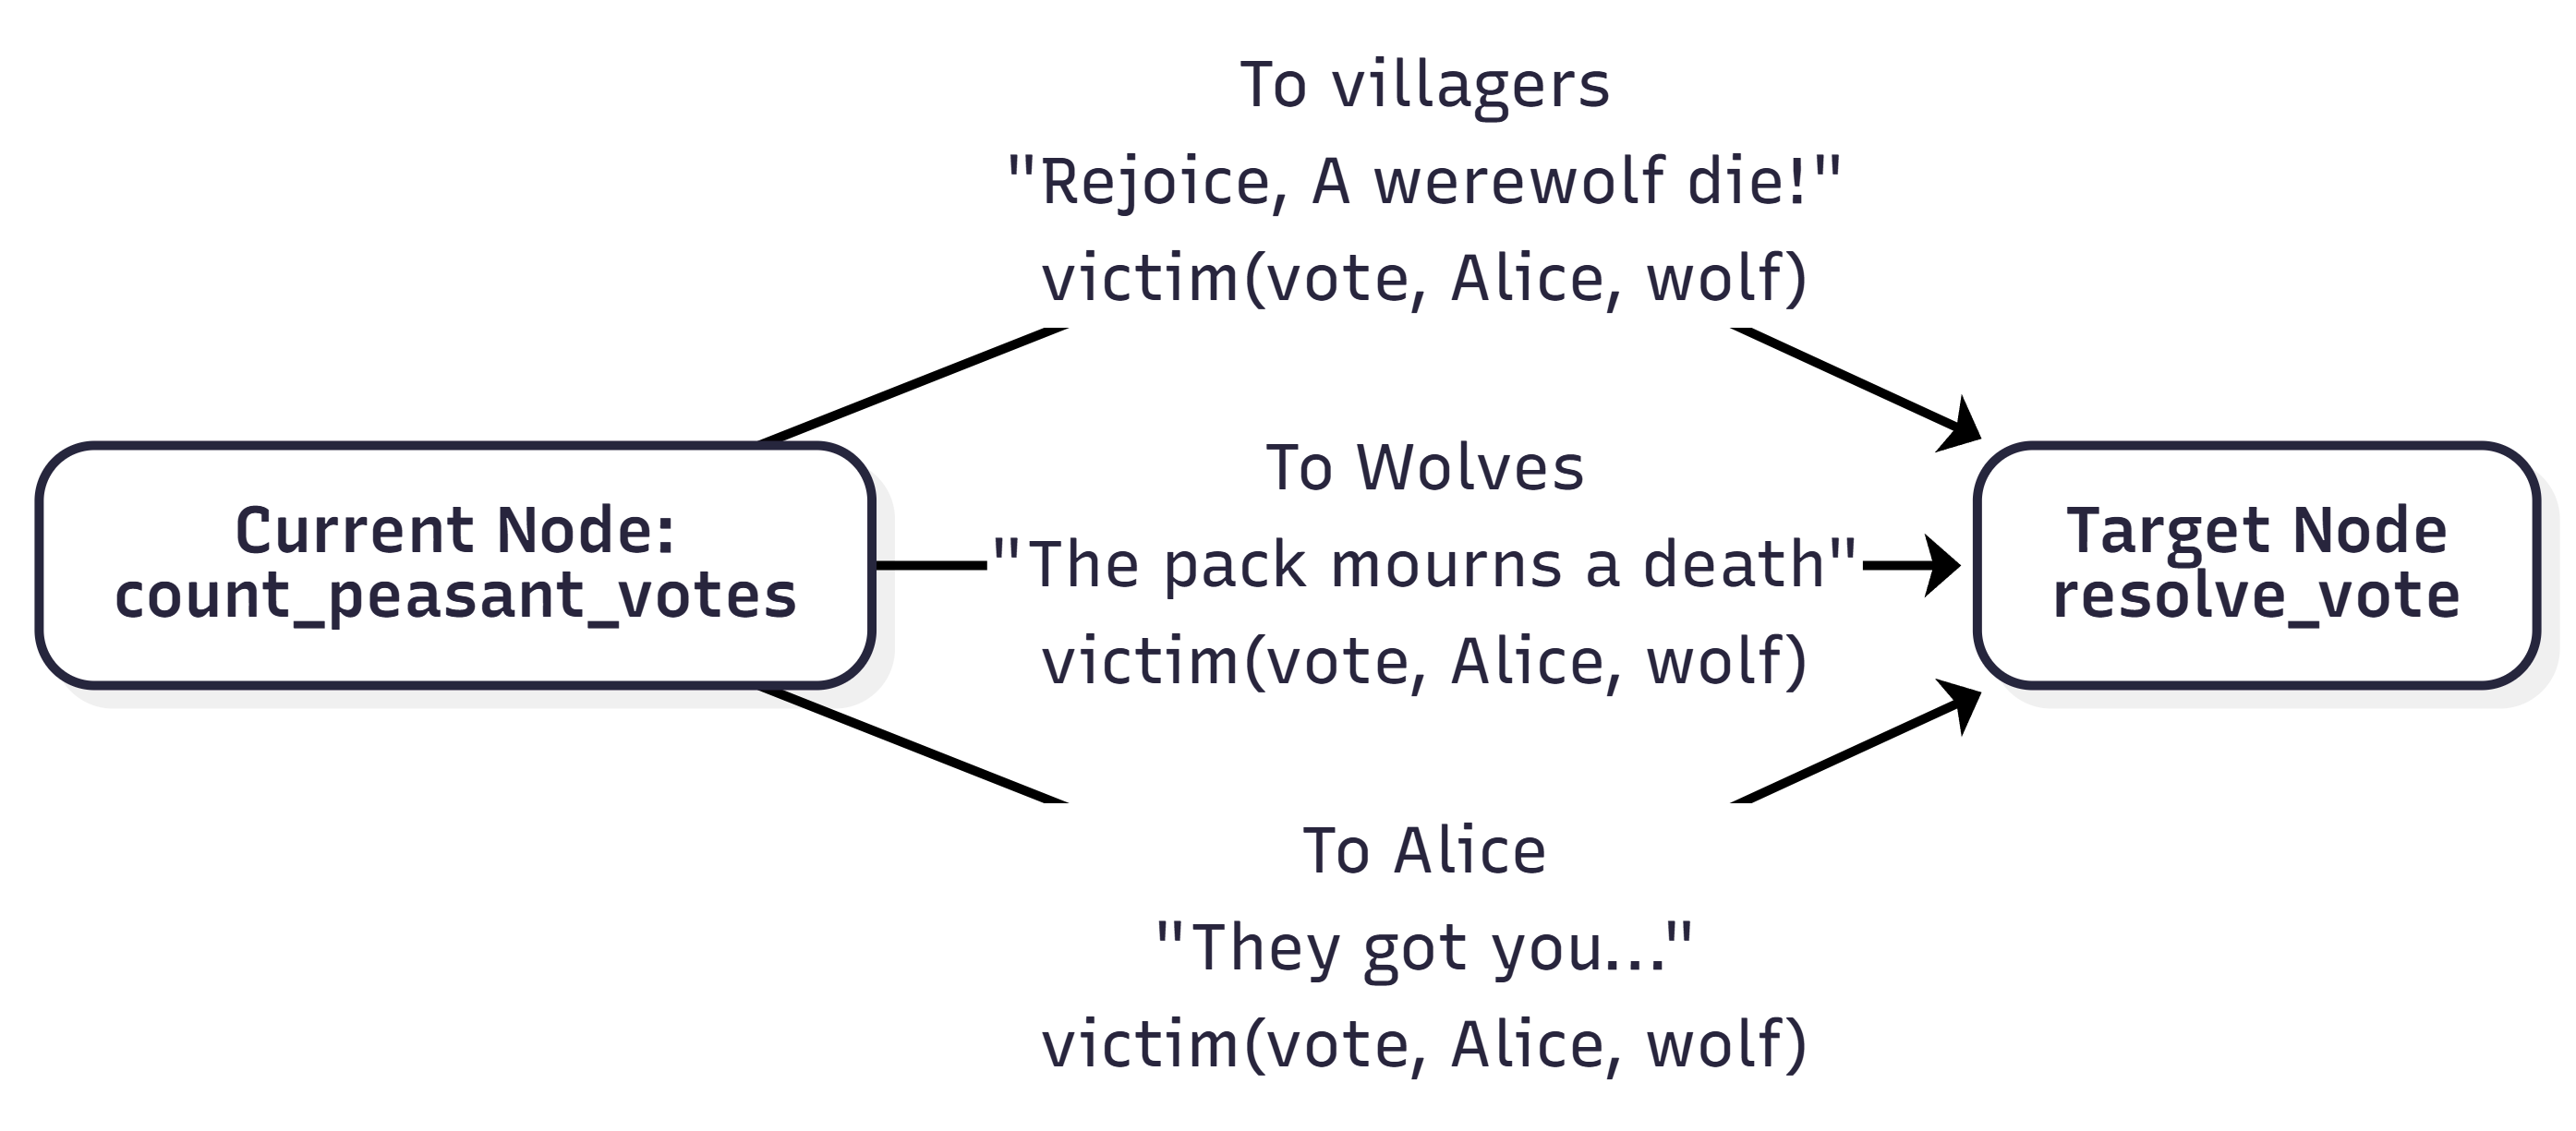
\includegraphics[width=\textwidth]{images/edge example.png}
    \caption{Example of a edge with multiple instances that can be activated at the same time, used to communicate that the Daytime Voting Phase has ended with a victim; different messages are sent to different audiences.}
    \label{fig:edge example}
\end{figure}


\subsubsection{Executing the Transition}
The core phase progression is handled by the Narrator's \texttt{execute\_transition} plan, as illustrated in Figure \ref{fig:transition_sequence}.

The plan executes all the subroutines needed to change the belief base, to bridge between phases.
When a phase concludes, the transition is executed:

\begin{enumerate}
    \item \textbf{Edge Evaluation and Exit:} The Narrator evaluates the current beliefs to select a valid outgoing \texttt{edge}. It then triggers the \texttt{ExitAction} of the current node to clean up the outgoing state.
    
    \item \textbf{Broadcast and Dispatch:} The Narrator extracts all valid \texttt{msg} payloads associated with the evaluated transition. It iterates through this collection and dispatches each payload to the specified \texttt{Players}\footnote{The players' reactions to these goals injected into their goal base are thoroughly explained in Section~\ref{sec:players}.}.
    
    \item \textbf{Node Entry and Synchronization:} The Narrator evaluates the new node's entry definition. If an explicit \texttt{EnterAction} is defined, the Narrator dispatches this action to the specified \texttt{Players} (e.g., instructing them to cast a vote) and immediately erects a \textbf{Synchronization Barrier} (detailed in Section \ref{subsec:sync-barrier}). The Narrator halts its internal game loop, waiting until it receives the corresponding \texttt{sync\_reply} responses from all targeted agents before proceeding. If no entry action is defined, the Narrator bypasses the barrier and directly executes the node's internal logic.
\end{enumerate}

\begin{lstlisting}[frame=single, language=Prolog, caption={Simplified Jason logic for the Narrator's transition engine (UI/LLM logics are removed for sempliticy).}, label={lst:transition_engine_code}]
+!execute_transition 
    : current_node(CurrentNode) 
    & edge(CurrentNode, _, NextNode)
    <-  !process_transition(CurrentNode, NextNode).

+!process_transition(CurrentNode, NextNode)
    <-  .findall(OutgoingMsg, 
            edge(CurrentNode, OutgoingMsg, NextNode), 
            AllMessages);
        
        ?node(_, CurrentNode, CleanupList);
        for ( .member(StaleBelief, CleanupList) ) 
        { .abolish(StaleBelief); };
        
        !activate_node(NextNode, AllMessages).

+!activate_node(NodeName, AllMessages)
    <-  -+current_node(NodeName);        
        for ( .member(OUT, AllMessages) ) {
            if (OUT = msg(TargetList,
                    BaseMessage, PhaseTitle, PhaseIntent, 
                    Actions_to_log)
                ) {
                
                !dispatch_phase(
                    TargetList, NodeName, 
                    PhaseTitle, BaseMessage);
                    
                for ( .member(Action, Actions_to_log) ) 
                { !dispatch_action(TargetList, Action); };
                
            };
        };

        ?node(IN, NodeName, _);
        if (IN = action(ActionTargets, Action)) {
            -+waiting_on(ActionTargets);
            .send(ActionTargets, achieve, Action);
        } else {
            !NodeName;
        }.
\end{lstlisting}

\begin{figure}[H]
    \centering
    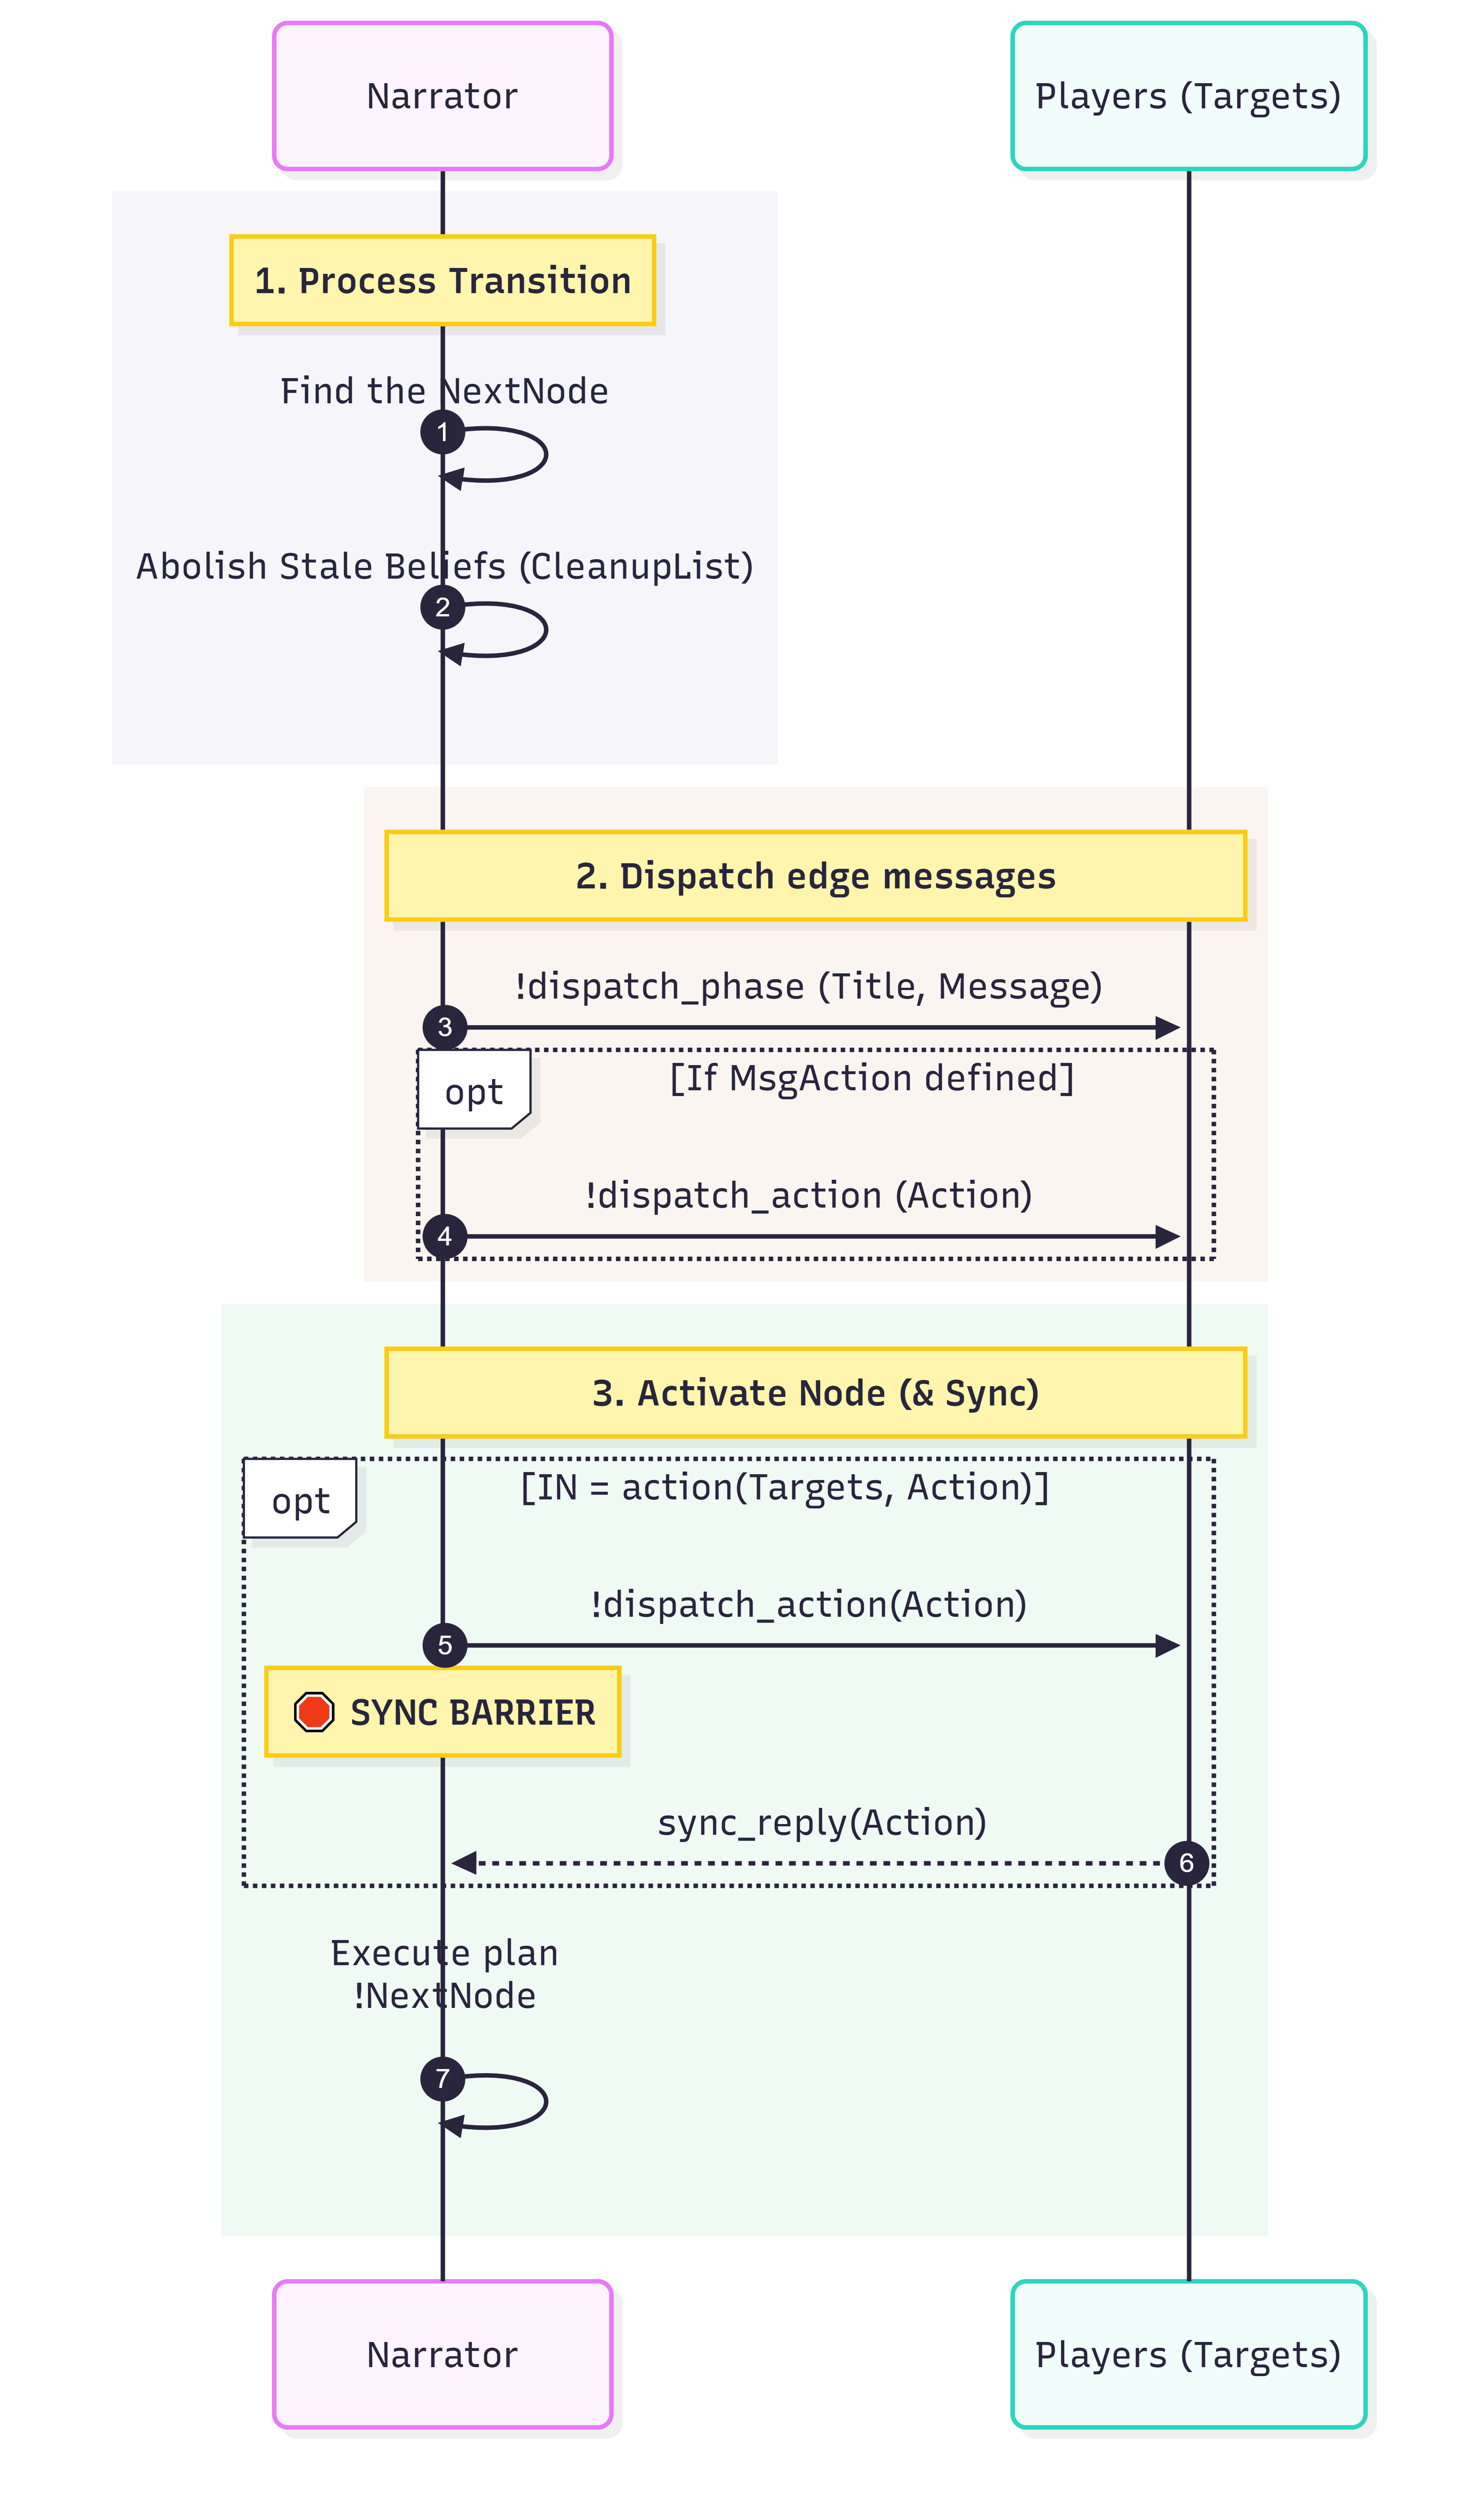
\includegraphics[width=\textwidth, height=0.95\textheight, keepaspectratio]{images/transition_phase_diagram.png}
    \caption{Sequence diagram illustrating the \texttt{execute\_transition} logic: the narrator can be halted in until some specific player responds to it, to synchronize their state.}
    \label{fig:transition_sequence}
\end{figure}



\subsection{Synchronization Barrier}
\label{subsec:sync-barrier}

Because the game relies entirely on message exchange and logical states, preventing race conditions and desynchronization between agents is critical\footnote{In this context, utilizing an engine explicitly optimized for proactivity, such as Jason, is arguably a disadvantage. It needs the implementation of slow, custom-built synchronization barriers that \emph{de facto} nullify the agents' proactive capabilities.}. If agents were allowed to send actions to the Narrator or to each other at any arbitrary time, the Multi-Agent System would quickly fall into an invalid state (e.g., an agent attempting to cast a vote while another is still finishing a speech). 

Furthermore, unregulated message broadcasting would result in agents observing and reacting to game events in different chronological orders: this temporal misalignment would inevitably corrupt their reasoning processes and destroy their ability to strategically align with one another.

To solve this, the architecture strictly enforces a unidirectional flow of control: \textbf{players are entirely reactive}. The \emph{only} way for a player to communicate an action back to the Narrator is by replying to a specific prompt using the \texttt{sync\_reply(Payload)} performative. 

\subsubsection{Technical implementation}
When the Narrator enters a node that requires player interaction (e.g., an \texttt{EnterAction} like \texttt{action(Targets, choose\_vote)}), it generates a \texttt{waiting\_on(Targets)} belief containing a list of all authorized agents. The internal graph traversal halts, and the Narrator becomes a passive listener waiting for \texttt{sync\_reply} messages.

\vspace{1em}
\begin{lstlisting}[frame=single, language=Prolog, caption={The Synchronization and Payload Management mechanics from the narrator; it is passively waiting for external messages from the players.}, label={lst:sync_logic}]
@sync_handler[atomic]
+!sync_reply(Payload)[source(Sender)]
    : waiting_on(WL) & .member(Sender, WL) 
    <-  +Payload;
        !manage_sync_payload(Payload);
        .delete(Sender, WL, NewWL);
        if (NewWL == []) {
          -waiting_on(_);
          !execute_transition;
        } else {
          -+waiting_on(NewWL);
        }.

//Example: votes are managed by mirroring them to all agents
+!manage_sync_payload(vote(Voter, Target)) 
    : players(AllPlayers)
    <-  !dispatch_action(AllPlayers, vote(Voter, Target)).
\end{lstlisting}

The resolution of this barrier operates in three distinct steps, as defined in the Jason logic (Listing \ref{lst:sync_logic}):

\begin{enumerate}
    \item \textbf{Sender validation:} When a \texttt{sync\_reply} arrives, the Narrator first verifies that the sender is currently in the \texttt{waiting\_on} list. If valid, the payload is accepted and the sender is removed from the list (if a player response, even if it is not on the waiting  list, something is irremediably wrong).
    
    \item \textbf{Payload Management \& Dispatch:} The narrator then processes the received payload (e.g., a vote or a speech from a player) via \texttt{manage\_sync\_payload}\footnote{Is overloaded in the plan base, and at runtime is called the suitable one; unexpected payloads are correctly notified.}. The Narrator explicitly dispatches this payload as an \texttt{action} to all relevant players in the game. This ensures that every player manages the event in the same order, maintaining the Narrator as the absolute single source of truth and avoiding P2P communications.
    
    \item \textbf{Barrier Release:} Once the \texttt{waiting\_on} list becomes completely empty, the Narrator destroys the barrier belief and safely resumes the graph traversal by calling \texttt{!execute\_transition} to proceed to the next node.
\end{enumerate}


Figure \ref{fig:sync_sequence} visualizes this exact flow, demonstrating how the Narrator processes concurrent replies while maintaining global synchronization through intermediate dispatching.

\begin{figure}[H]
    \centering
    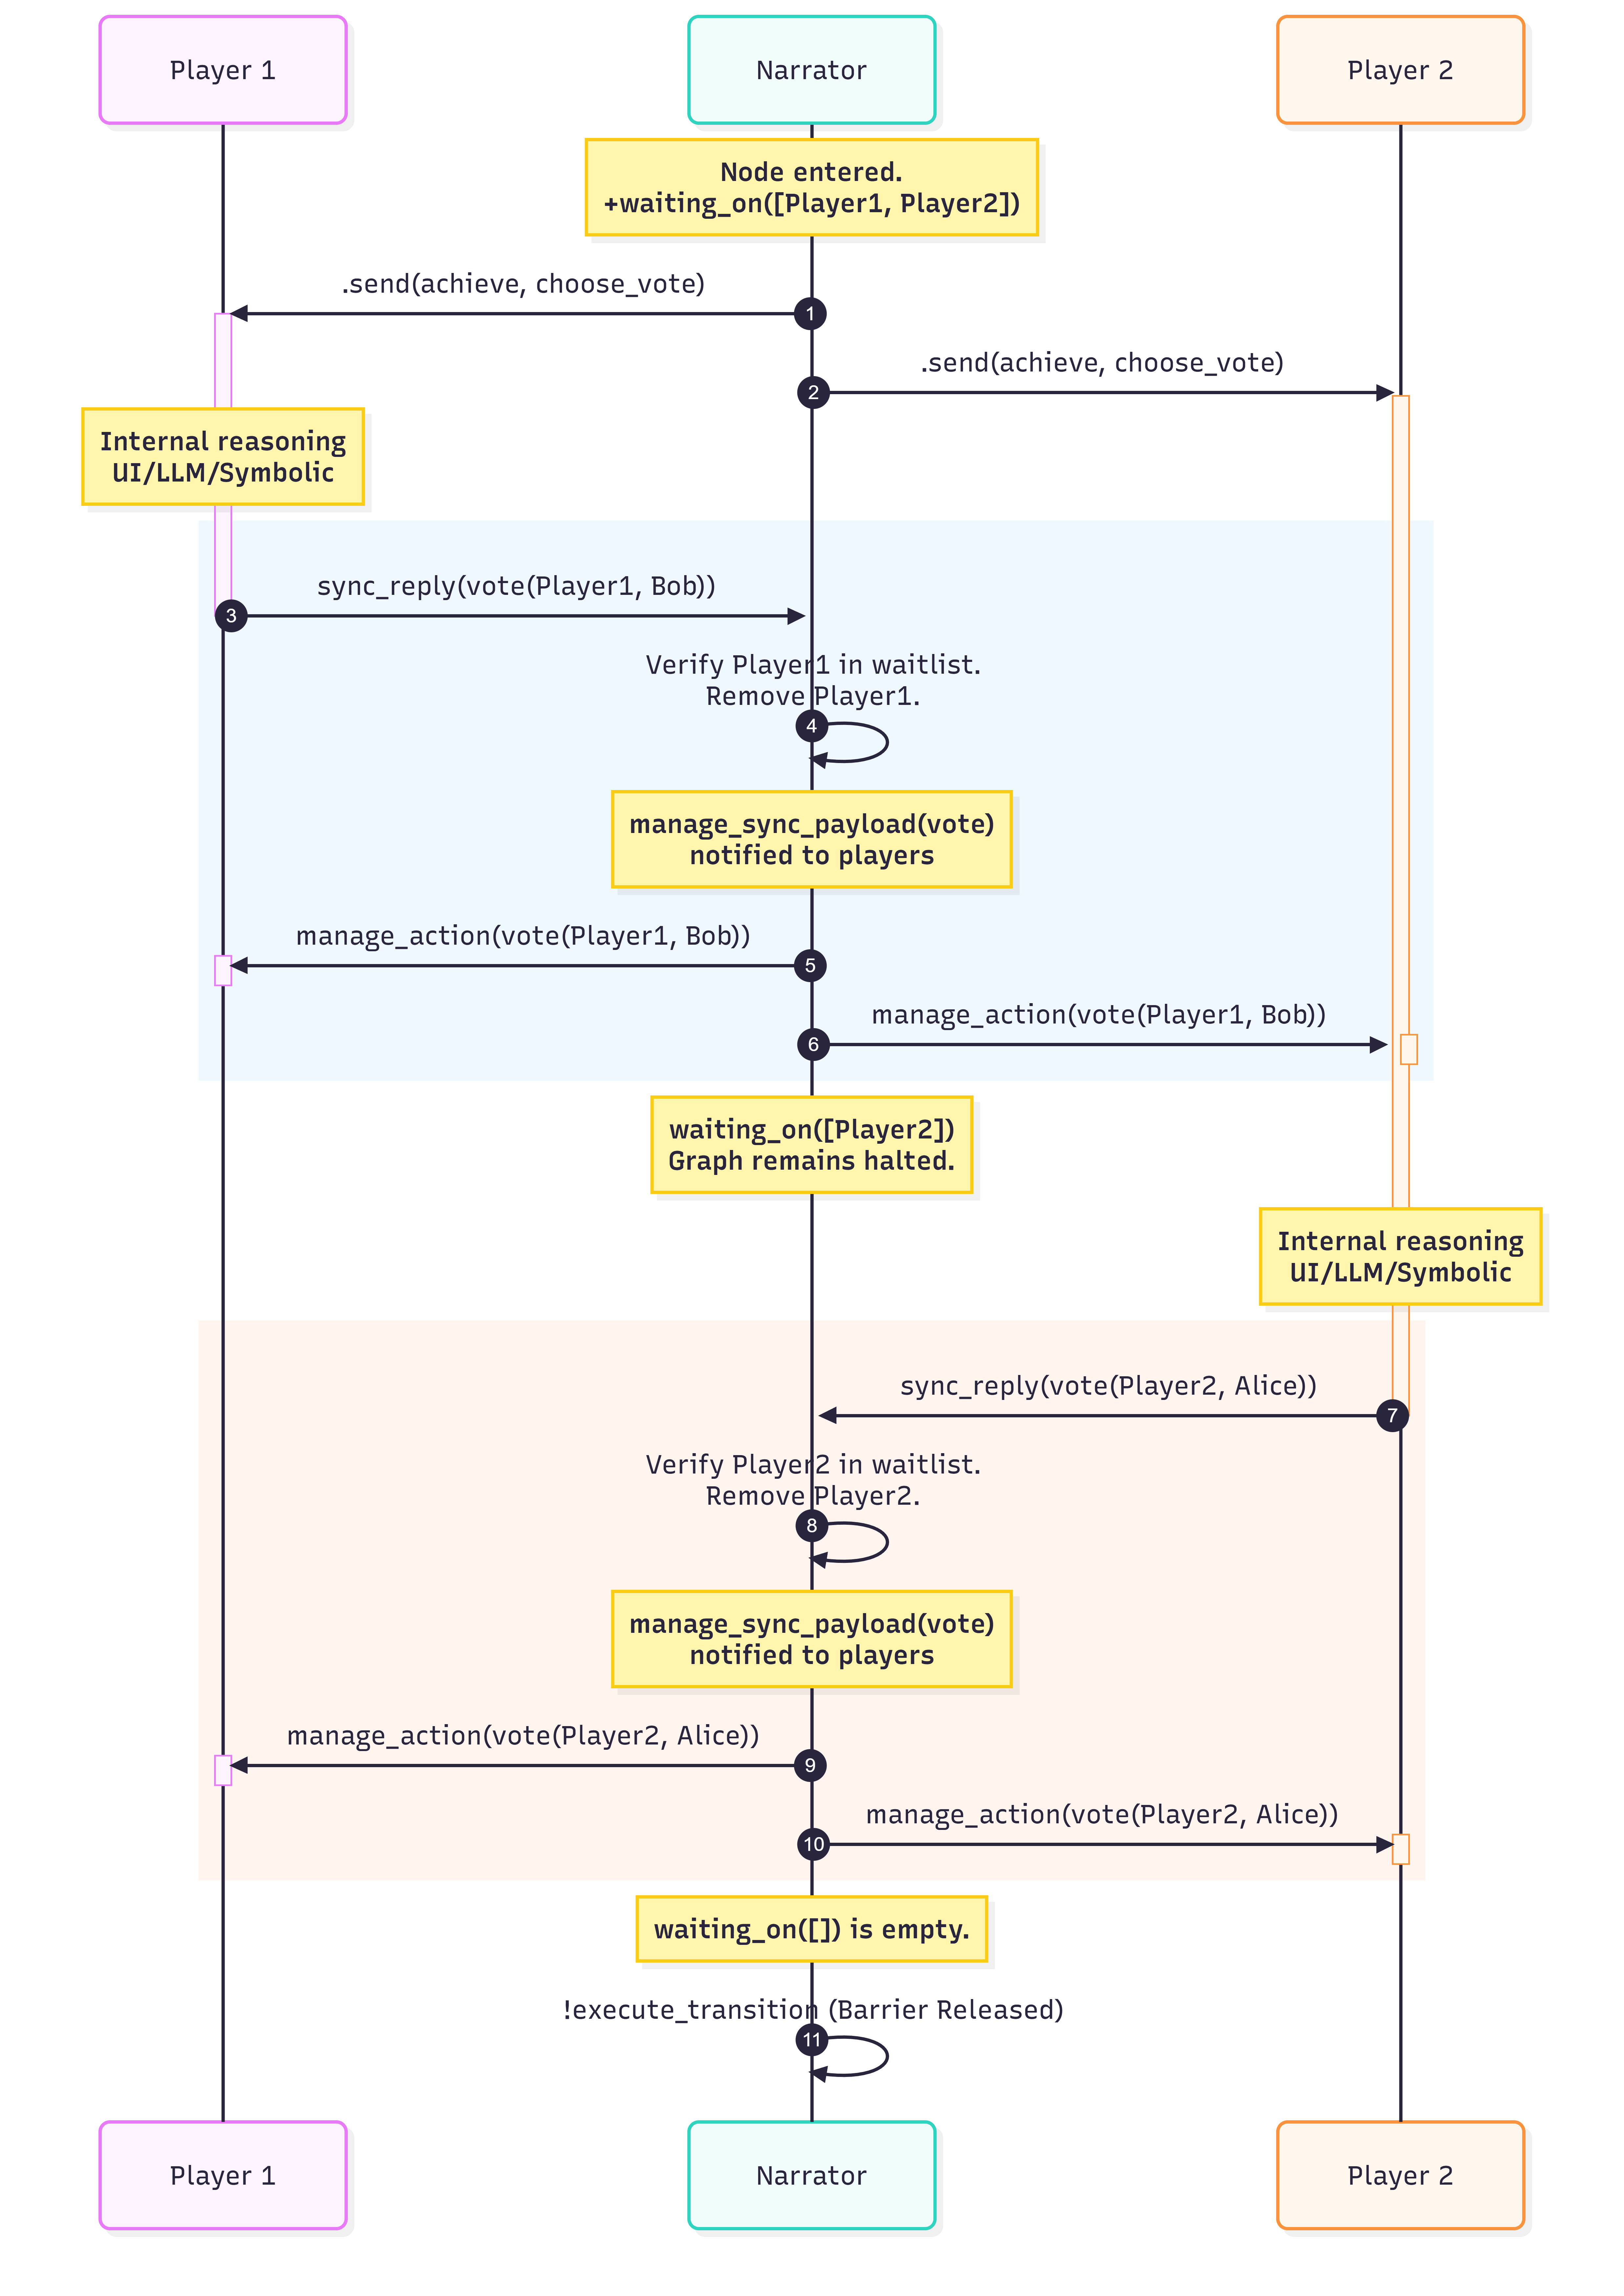
\includegraphics[width=1\textwidth]{images/sync_barrier_diagram.png}
    \caption{Sequence diagram illustrating the resolution of the Synchronization Barrier. The primary objective is to guarantee that the Narrator and all active players ultimately maintain an identical, globally synchronized chronological log of events (e.g., \texttt{choose\_vote}, \texttt{vote(Player1, bob)}, \texttt{vote(Player2, alice)}).}
    \label{fig:sync_sequence}
\end{figure}




\subsection{Phase Execution Examples}
\label{subsec:phase-execution-examples}

While the general transition engine manages the flow of the Game Graph, some specific nodes require the Narrator to execute custom logic to resolve the game state; this section details the \emph{vote counting} and the \emph{speaker selection} practical implementation.

\subsubsection{Vote Counting Mechanism}
The voting counts mechanism is used in particular twice in the game logic :after  the Wolves' nocturnal hunt and the Villagers' daytime execution.
The Narrator triggers either \texttt{count\_hunt\_votes} or \texttt{count\_peasant\_votes}, which collects all the respective vote beliefs; then to ensure reusability, the target's list is unified with a goal-oblivious Prolog rule \texttt{tally\_votes}.


\vspace{1em}
\begin{lstlisting}[frame=single, language=Prolog, caption={The unified vote counting logic and the \emph{Peasant vote} resolution plan; after the count, \texttt{tie\_count\_village(TieCount)} indicates if the vote was a tie, and \texttt{max\_victim\_village(MaxVictim)} defines the eventual victim of the vote.}, label={lst:vote_counting}]
tally_votes(VoteList, TieCount, MaxVictim)  
    :-.setof(V, .member(V, VoteList), UniqueVictims)          
    & .findall(vote_count(C, V),
        ( .member(V, UniqueVictims) 
        & .count(.member(V, VoteList), C)), 
        Tally)
    & .max(Tally, vote_count(MaxCount, MaxVictim))            
    & .count(
        .member(vote_count(MaxCount, _), Tally), 
        TieCount). 

+!count_peasant_votes
    <-  .findall(V, vote(_, V), AllVotes);
        ?tally_votes(AllVotes, TieCount, MaxVictim);
        
        //save results as beliefs
        +tie_count_village(TieCount); 
        +max_victim_village(MaxVictim);
        
        !execute_transition.
\end{lstlisting}

The \texttt{tally\_votes} rule then processes the list through as shown in Listing \ref{lst:vote_counting}:
\begin{enumerate}
    \item It extracts a set of all unique targeted victims.
    \item It counts the occurrences of each target within the vote list.
    \item It define the highest vote count and the specific victim who received it.
    \item It checks how many targets receive the maximum number of votes.
\end{enumerate}

The count's results are then saved as explicit beliefs: they will be automatically used by the Jason Interpreter to define wich edges are valid, during the explicitly called transition to the  next phase. 

\subsubsection{Speaker Selection Implementation}
\label{subsubsec:speaker_selection}

During the \texttt{start\_discussion\_round} phase, players explicitly tell the Narrator their intent to speak based on their internal reasoning. The Narrator then chooses (simulating a natural conversation, while avoiding monopolization) from those volunteers a Player that hold the floor.

Upon entering the \texttt{evaluate\_intents\_to\_speak} node, the Narrator collects all volunteer intents and categorizes them to ensure a responsive and logically coherent dialogue. These categories carry the following semantic meanings:

\begin{itemize}
    \item \textbf{\texttt{yes} (\texttt{normal}):} The player is an AI (symbolic or LLM) that wants to speak.
    \item \textbf{\texttt{privileged}:} Human players with intents to speak. Prioritizing their inputs augment human interactivity and overall game enjoyability.
    \item \textbf{\texttt{targeted}:} Specific player who was the direct topic of the preceding speech in the current round; it has a higher chance to be choosen to speak, to ensure the  possibility to defend  itself from previous accusations.
\end{itemize}
To enforce a dynamic dialogue, the Narrator explicitly filters out the \texttt{last\_speaker} from all eligibility lists, ensuring no player can speak twice in a row in the same round. 

\vspace{1em}
\begin{lstlisting}[frame=single, language=Prolog, caption={The priority cascade logic for speaker selection, with 4 rules evaluated top to bottom. The arguments needed are list of the players with intent to speak, subdivided in Privileged, Targeted, Normal}, label={lst:speaker_selection}]

// Priority 1: Privileged volunteer (Human players)
+!pick_candidate(Privileged, _, _, Speaker) 
    : Privileged \== []
    <- .shuffle(Privileged, [Speaker|_]).

// Priority 2: Targeted player (P=0.25)
+!pick_candidate(_, [Speaker], _, Speaker) 
    : .random(R) & R <= 0.25.

// Priority 3: Normal volunteer (AI agents)
+!pick_candidate(_, _, Normal, Speaker) 
    : Normal \== []
    <- .shuffle(Normal, [Speaker|_]).

// Priority 4: Targeted player
+!pick_candidate(_, [Speaker], _, Speaker).
\end{lstlisting}

If no one volunteers (meaning both the normal and privileged lists are empty), the Narrator immediately aborts the discussion round; otherwise, the selection process follows a priority cascade defined by the\texttt{pick\_candidate} plans, detailed in Listing \ref{lst:speaker_selection}:

\begin{enumerate}
    \item \textbf{Human players :} If any active human player define the intent to speak, sample one randomly. 
    \item \textbf{Right to fight back:} If the previously targeted player wishes to speak, with chances of 25\% it will hold the floor.
    \item \textbf{Random selection:} Select randomly (if any) a Agent driven by its AI, with positive intent to speak.
    \item \textbf{Duty to fight back:} Fallback case, the floor is given to the targeted player by default.
\end{enumerate}

Once a speaker is designated, the Narrator logs them as the new \texttt{last\_speaker}, broadcasts a \texttt{time\_to\_speak} action to all players, and sets up a synchronization barrier waiting specifically for that agent to deliver their speech payload.

\subsection{Logging System}
\label{subsec:logging}

The Narrator manages a centralized \emph{log} to keep a persistent history of the game (the logic is self-contained in the file \texttt{narrator/log\_manager/logger.asl}). Before dispatching any phase transition or action to the agents, the engine internally appends it to this log (with an $O(1)$ complexity, since it is natively implemented as a linked list). 

The list is used in an append-only fashion: new entries are pushed to the head, and entries are never removed, only retrieved when needed\footnote{This inherent inability to cut off past events even if they are no longer useful could theoretically lead to memory-related problems, but in practice, no tests ever reached that critical point.}.

To prevent knowledge leakage (e.g., ensuring a Villager cannot access the Wolves' nocturnal chat), we exploit Jason's native belief annotations. Every entry is tagged with its specific audience. 
To optimize RAM usage and improve readability, the actual list of targets is compressed into global keywords (\texttt{players}, \texttt{wolves}, \texttt{villagers}) when possible before being stored. 

When an agent needs to retrieve a chunk of the log\footnote{The use cases of the retrieval system are explained in Section~\ref{sec:llm}: the log is used to further drive of the \emph{in-context learning} natively implemented by the LLM.}, it can directly query the Narrator: the compressed annotations are expanded back into a list, and the Narrator verifies if the requesting set of players is a valid subset of the entry's audience (if not, the entry is simply ignored). 

This centralized extraction logic prevents the extreme RAM usage that would occur if we maintained separate, parallel logs for every single player in the MAS.